\section{Focus of this Thesis Work}
A surgery consists of a series of subtasks, some suited for robotized autonomous execution. Prior work in motion planning and control of subtasks for surgical robots include knot tying, suturing and more advanced statistical learning of subtasks from recording surgeon motions \citep{bib:raven_debride,bib:raven_observ}.

This report presents the work on a guaranteed safe end-effector setpoint control, %. As opposed to the safety control by virtual potential field constraints \citep{bib:dlr_miro}, this work utilizes 
utilizing the barrier certificate method where the robot is physically prevented from entering unsafe areas thereby guaranteeing safety \citep{bib:safety}. A short overview of the controller is given in \autoref{sec:project_overview}.

The algorithm is tested on a first generation da Vinci surgical robot, detached from its surgeon controller console and modified to be controllable by automated processes. An overview of the system is given in \autoref{sec:technical_overview}.


%One should certainly take the risk of patient trauma when an automated surgery is conducted into account. This is seen in Therac-25. 



\subsection{Technical Overview of the Robotic Surgery System}\label{sec:technical_overview}
A simplified overview of the robot controller setup is provided in \autoref{fig:overview}. The setup is physically located at the Control and Automation laboratory at Aalborg University. 

\Autoref{fig:overview} is structured in descending abstraction layers with the highest at the top (i.e. the \gls{ros} - an open source software framework for robots \citep{bib:ros}, see \autoref{app:ros} for further details), which establishes a wireless TCP/IP communication channel receiving all positions from the robot as feedback and produces position control signals to the NI (National Instruments) single board \glspl{rio} which handle all input/output communication with the user. The NI single board \glspl{rio} consist of a primary and a secondary board. The reason for having two \gls{rio} boards is solely the lack of input/outputs on one board.

The \gls{rio} boards direct the control signals to a cascaded controller taking in the position reference from the user and delivering a current control signal to the ESCON motor driver. The velocity and current controllers are implemented in \gls{fpga} based hardware to ensure sufficient controller speed relative to the system \citep{bib:robot_paper}. The ESCON motor driver manages advanced processing and essentially delivers an appropriate PWM signal for the actuators (seven Maxon motors) which represent the lowest abstraction layer, located at the bottom of the figure.

The NI single board \glspl{rio} concurrently handle most safety precautions and enabling/disabling movement of the arm itself (see \autoref{app:links_joints_3d} and \ref{app:kinematic_model_robot} for an overview of the arm and its kinematics, respectively) through solenoids.
\begin{figure}[H]
\hspace*{-5mm}
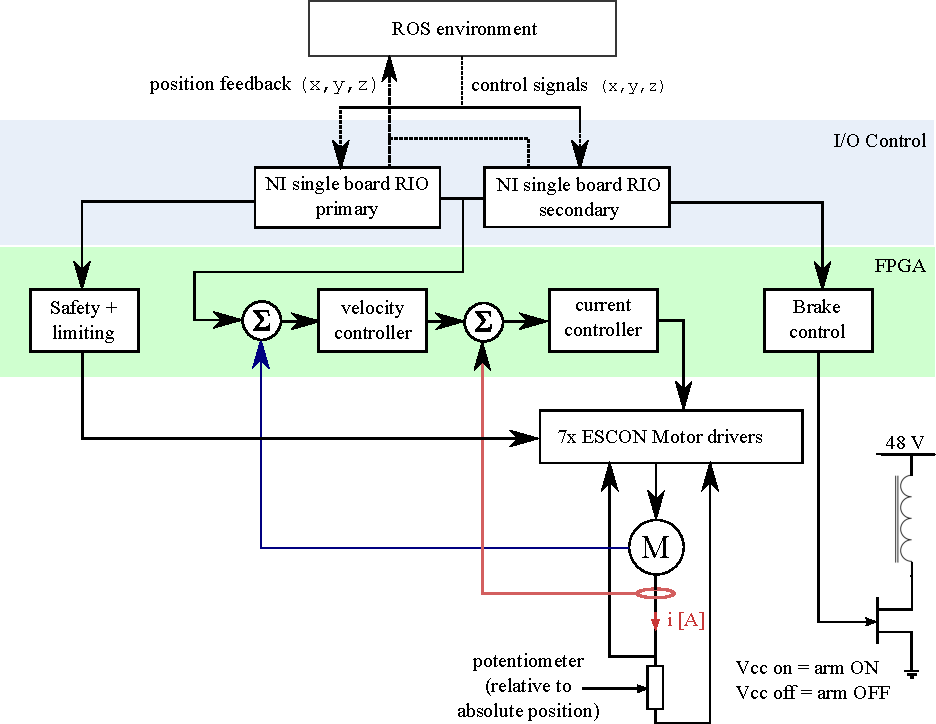
\includegraphics[width=1.1\textwidth]{overview.pdf}	
\caption{Overview of the custom made hardware and controllers for the 1st generation da Vinci surgical robot located at Aalborg University's department of Control and Automation.}
\label{fig:overview}
\end{figure}

In order to prevent potential violation of physical joint constraints, stricter constraints on each joint position are set in the low-level motor controllers, that disable the controller if exceeded.


\subsection{Overview of Thesis Contribution to the AAU da Vinci System}\label{sec:project_overview}
The focus of this thesis is the highest abstraction layer as seen in the top of \autoref{fig:overview}, i.e. the ROS environment. The purpose of this layer primarily constitutes the implementation of algorithms that require heavy processing and non real-time processing or tasks with loose timing constraints \citep{bib:robot_paper}.
This pool of stipulations essentially and practically entails the following main topics of this thesis:
\begin{itemize}
\itemsep-1.3mm
	\item User input in the form of desired final end-effector (position) setpoints
	\begin{itemize}
		\vspace*{-1mm}
		\item in fixed space
		\item relative to a point on the surface of a beating heart
	\end{itemize}
%	\item Static trajectory planning from current to final position enforcing safety by means of barrier certificates.
	\item Control of setpoint (position) tracking 
	\begin{itemize}
		\vspace*{-1mm}
		\item with static boundaries for safe and unsafe regions, controller safety guaranteed by barrier certificates
		\item with dynamic boundaries for safe and unsafe regions,  such as the surface of a beating heart, controller safety guaranteed by barrier certificates
	\end{itemize}
\end{itemize}



%Raven-II inverse control process (not primarily to estimate the pose, in which case standard estimation methods like Kalman would be appropriate) is to calculate, give an desired true pose, the input pose to send the control sw to reach the desired true pose (detected pose with vision system assumed to be the true pose), estimate between measurements using updates from forward kinematics \citep{bib:raven_debride}.

%advances in motion planning, control and perception: integrated task and motion planning ofhigh level task planning using state machines, and motion planning for low level planning algorithm  \citep{bib:raven_debride}

%da Vinci Research Kit: learning from demonstrations/by observation. Targets considered form convex regions spherical/linear. \citep{bib:raven_observ}.